\documentclass[aspectratio=169,10pt]{beamer}

% --- Paquetes de Idioma y Tipografía ---
\usepackage[spanish,es-tabla,es-nodecimaldot]{babel}
\usepackage[utf8]{inputenc}
\usepackage[T1]{fontenc}
\usepackage{lmodern}
\usepackage{amsmath}
\usepackage{amssymb}
\usepackage{graphicx}
\usepackage{booktabs}
\usepackage{tabularx}

\graphicspath{{img/}}

% --- Tema Visual Institucional ---
\usetheme{Madrid}
\usecolortheme{whale}
\definecolor{primaryblue}{RGB}{0, 70, 140}
\definecolor{darkblue}{RGB}{10, 45, 95}
\definecolor{alertred}{RGB}{180, 20, 20}
\definecolor{okgreen}{RGB}{21, 128, 61}
\definecolor{lightgraybg}{RGB}{242, 245, 250}

\setbeamercolor{palette primary}{bg=primaryblue,fg=white}
\setbeamercolor{palette secondary}{bg=darkblue,fg=white}
\setbeamercolor{palette tertiary}{bg=darkblue,fg=white}
\setbeamercolor{structure}{fg=primaryblue}
\setbeamercolor{block title}{bg=primaryblue,fg=white}
\setbeamercolor{block body}{bg=lightgraybg,fg=black}
\setbeamercolor{block title alerted}{bg=alertred,fg=white}
\setbeamercolor{block title example}{bg=okgreen,fg=white}

\setbeamertemplate{navigation symbols}{}
\setbeamertemplate{caption}[numbered]

% --- Metadatos de Portada ---
\title[Infraestructura NAS — TIF]{Servidor de Almacenamiento Centralizado (NAS) y Servicios de Red}
\subtitle{Especificación, Seguridad SMB, Respaldos OpenZFS y Automatización GitOps\\Trabajo Integrador Final (TIF) — Soporte Técnico II}
\author[O. Meza y B. Riquelme]{\textbf{Autores:} Oriel Meza y Brisa Riquelme\\[0.15cm]\footnotesize Docente Evaluador: Lic. Pablo Nicolás Sasowski}
\institute[IESETyFP]{Instituto de Educación Superior de Educación Técnica y Formación Profesional (IESETyFP)}
\date{10 de noviembre de 2026}

\begin{document}

% ==============================================================================
% DIAPOSITIVA 1: PORTADA
% ==============================================================================
\begin{frame}
    \titlepage
\end{frame}

% ==============================================================================
% DIAPOSITIVA 2: ¿QUÉ ES UN NAS Y QUÉ PROBLEMA RESUELVE?
% ==============================================================================
\begin{frame}{1. ¿Qué es un servidor NAS y qué problema resuelve?}
    \framesubtitle{Expositora: Brisa Riquelme — Contexto operativo en el laboratorio escolar}
    \begin{columns}[T]
        \begin{column}{0.48\textwidth}
            \begin{block}{¿Qué es un NAS (\textit{Network Attached Storage})?}
                Es un servidor dedicado conectado a la red local (LAN) que centraliza el almacenamiento de archivos, permitiendo que múltiples computadoras (Windows y Linux) accedan a carpetas compartidas con permisos controlados por usuario.
            \end{block}
            \vspace{0.15cm}
            \begin{alertblock}{Problemática en aulas y laboratorios}
                \begin{itemize}
                    \item Trabajos prácticos dispersos en discos locales que se pierden o borran.
                    \item Ingreso constante de virus y ejecutables mediante pendrives.
                    \item Ausencia de copias de seguridad automáticas ante rotura de discos o cortes de luz.
                \end{itemize}
            \end{alertblock}
        \end{column}
        \begin{column}{0.49\textwidth}
            \begin{exampleblock}{Solución implementada en el proyecto}
                \begin{itemize}
                    \item \textbf{Almacenamiento en red SMB:} Carpetas para docentes, alumnos y directivos sin abrir puertos a Internet (0 puertos WAN).
                    \item \textbf{Aislamiento de entregas:} Buzón ciego donde ningún alumno puede ver ni borrar trabajos ajenos.
                    \item \textbf{Recuperación en 10 segundos:} El propio usuario restaura archivos borrados desde Windows (\textit{Versiones anteriores}).
                    \item \textbf{Administración web simple:} Alta de usuarios, planillas CSV y monitoreo desde navegador.
                \end{itemize}
            \end{exampleblock}
        \end{column}
    \end{columns}
\end{frame}

% ==============================================================================
% DIAPOSITIVA 3: ARQUITECTURA EN 4 PLANOS Y DASHBOARD GENERAL
% ==============================================================================
\begin{frame}{2. Arquitectura del Sistema y Panel de Estado General}
    \framesubtitle{Expositora: Brisa Riquelme — Organización en 4 planos técnicos aislados}
    \begin{columns}[T]
        \begin{column}{0.42\textwidth}
            \footnotesize
            \begin{enumerate}
                \item \textbf{Plano de Acceso (Samba SMB):} Expone las carpetas en red y traduce las instantáneas ZFS al explorador de Windows.
                \item \textbf{Plano de Control (K3s + Portal Web):} Gestiona cuentas, permisos y tareas en segundo plano (\texttt{TaskEngine}).
                \item \textbf{Plano de Persistencia (OpenZFS):} Pool \texttt{tank} en \textbf{RAID-Z1} (3 discos) con compresión \texttt{lz4} y verificación de integridad.
                \item \textbf{Plano de Continuidad:} Instantáneas cada 1 hora, agente \texttt{Sentinel} y copia cifrada a Cloudflare R2.
            \end{enumerate}
            \vspace{0.1cm}
            \textbf{En la captura:} Se observa la carga de CPU, uso controlado de RAM, estado \texttt{ONLINE} del pool ZFS y salida en vivo de \texttt{zpool status}.
        \end{column}
        \begin{column}{0.56\textwidth}
            \centering
            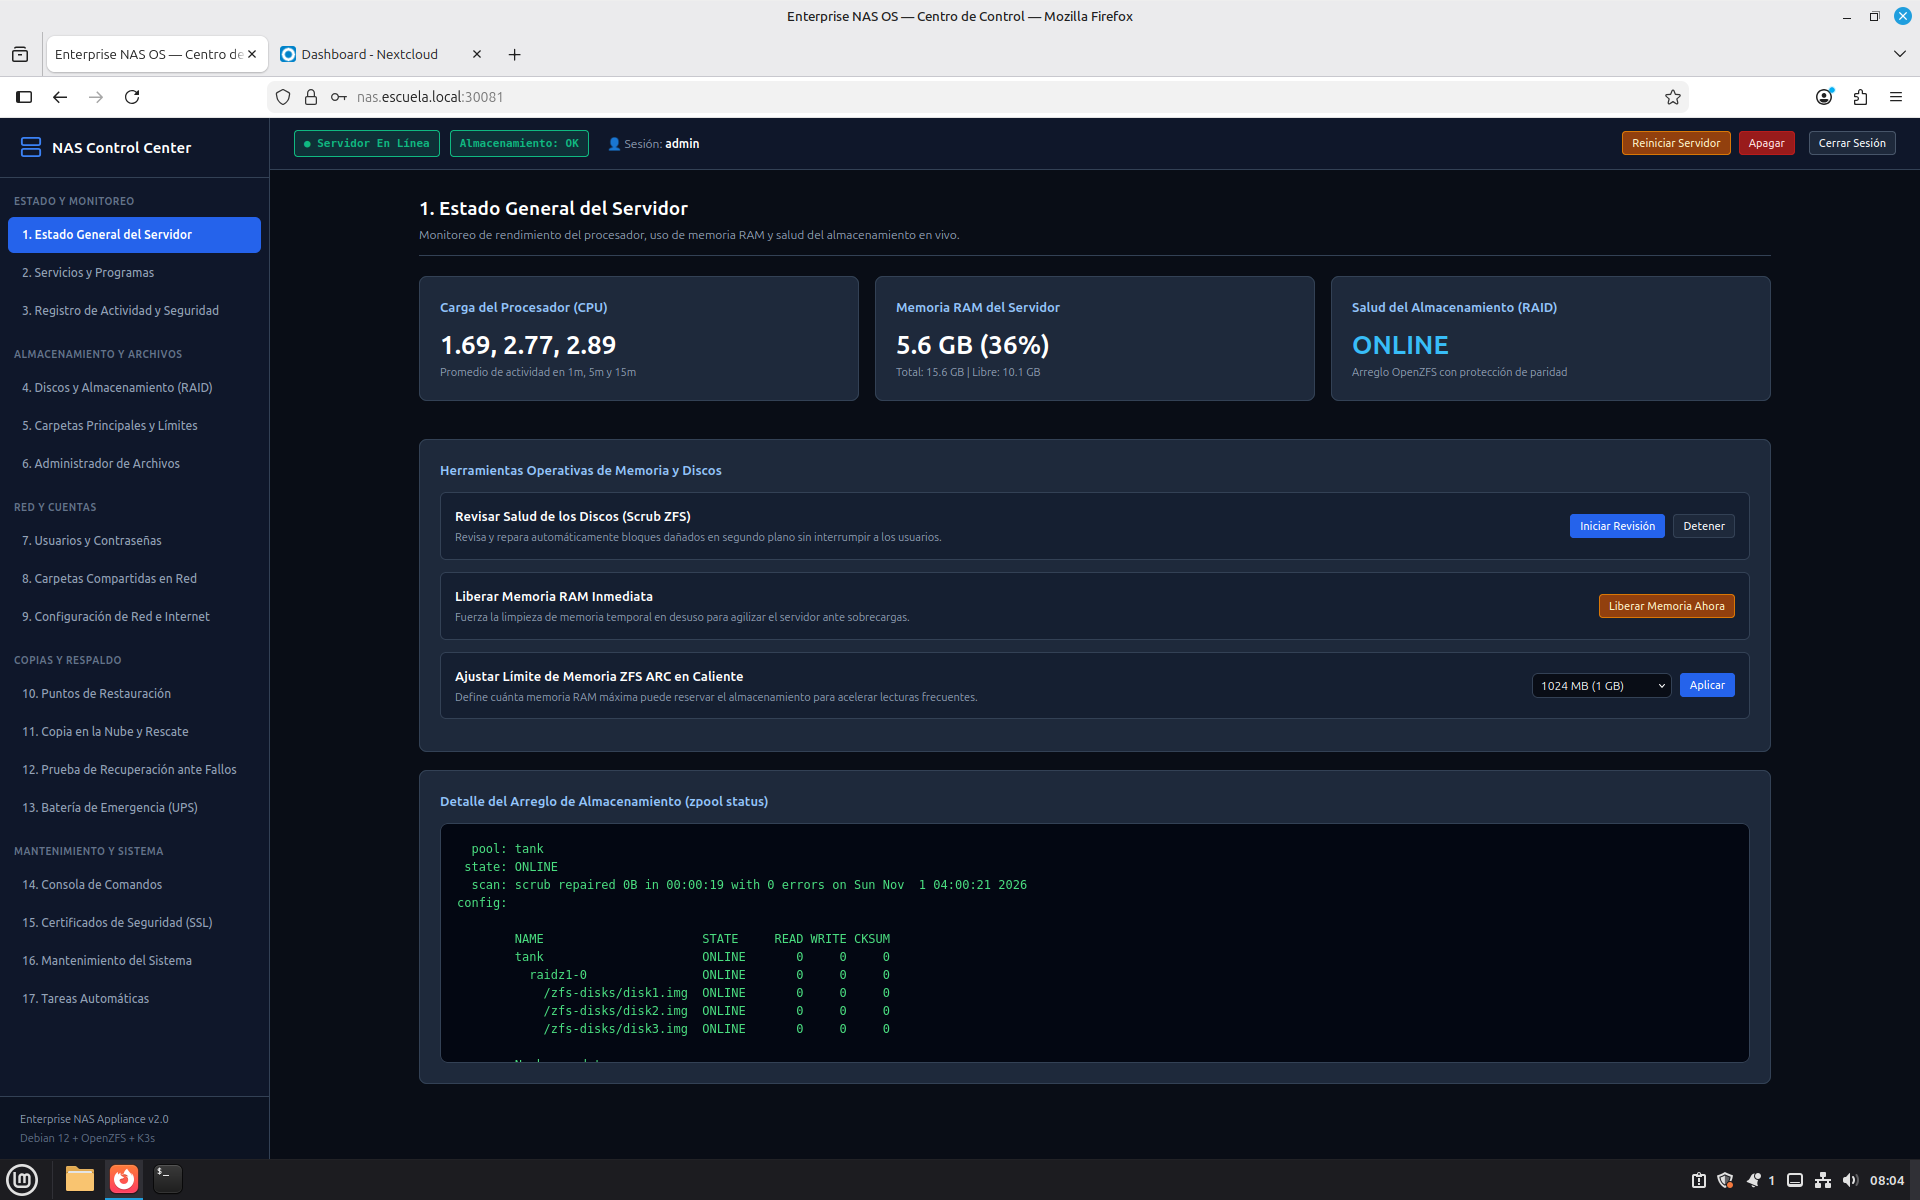
\includegraphics[width=\textwidth]{img/fig01_dashboard_general.png}
            \tiny Vista real del Centro de Control (\texttt{nas.escuela.local:30081}) — Sección 1: Estado General y \texttt{zpool status}.
        \end{column}
    \end{columns}
\end{frame}

% ==============================================================================
% DIAPOSITIVA 4: ¿QUÉ ES OPENZFS Y RAID-Z1?
% ==============================================================================
\begin{frame}{3. Almacenamiento OpenZFS y Tolerancia a Fallos (RAID-Z1)}
    \framesubtitle{Expositor: Oriel Meza — Protección frente a rotura física de discos y cortes de luz}
    \begin{columns}[T]
        \begin{column}{0.44\textwidth}
            \footnotesize
            \begin{block}{¿Qué es OpenZFS y por qué lo elegimos?}
                \begin{itemize}
                    \item \textbf{Copy-on-Write (CoW):} Nunca sobrescribe datos activos en el mismo bloque. Si hay un \textbf{corte abrupto de luz sin UPS}, el disco no se corrompe ni requiere \texttt{fsck}.
                    \item \textbf{RAID-Z1 (Paridad distribuida):} Combina 3 discos; tolera la \textbf{rotura física completa de 1 disco} sin interrumpir el servicio ni perder datos.
                    \item \textbf{Checksums Fletcher4 y Scrub:} Detecta degradación silenciosa (\textit{bit-rot}) y repara bloques automáticamente leyendo la paridad.
                \end{itemize}
            \end{block}
        \end{column}
        \begin{column}{0.54\textwidth}
            \centering
            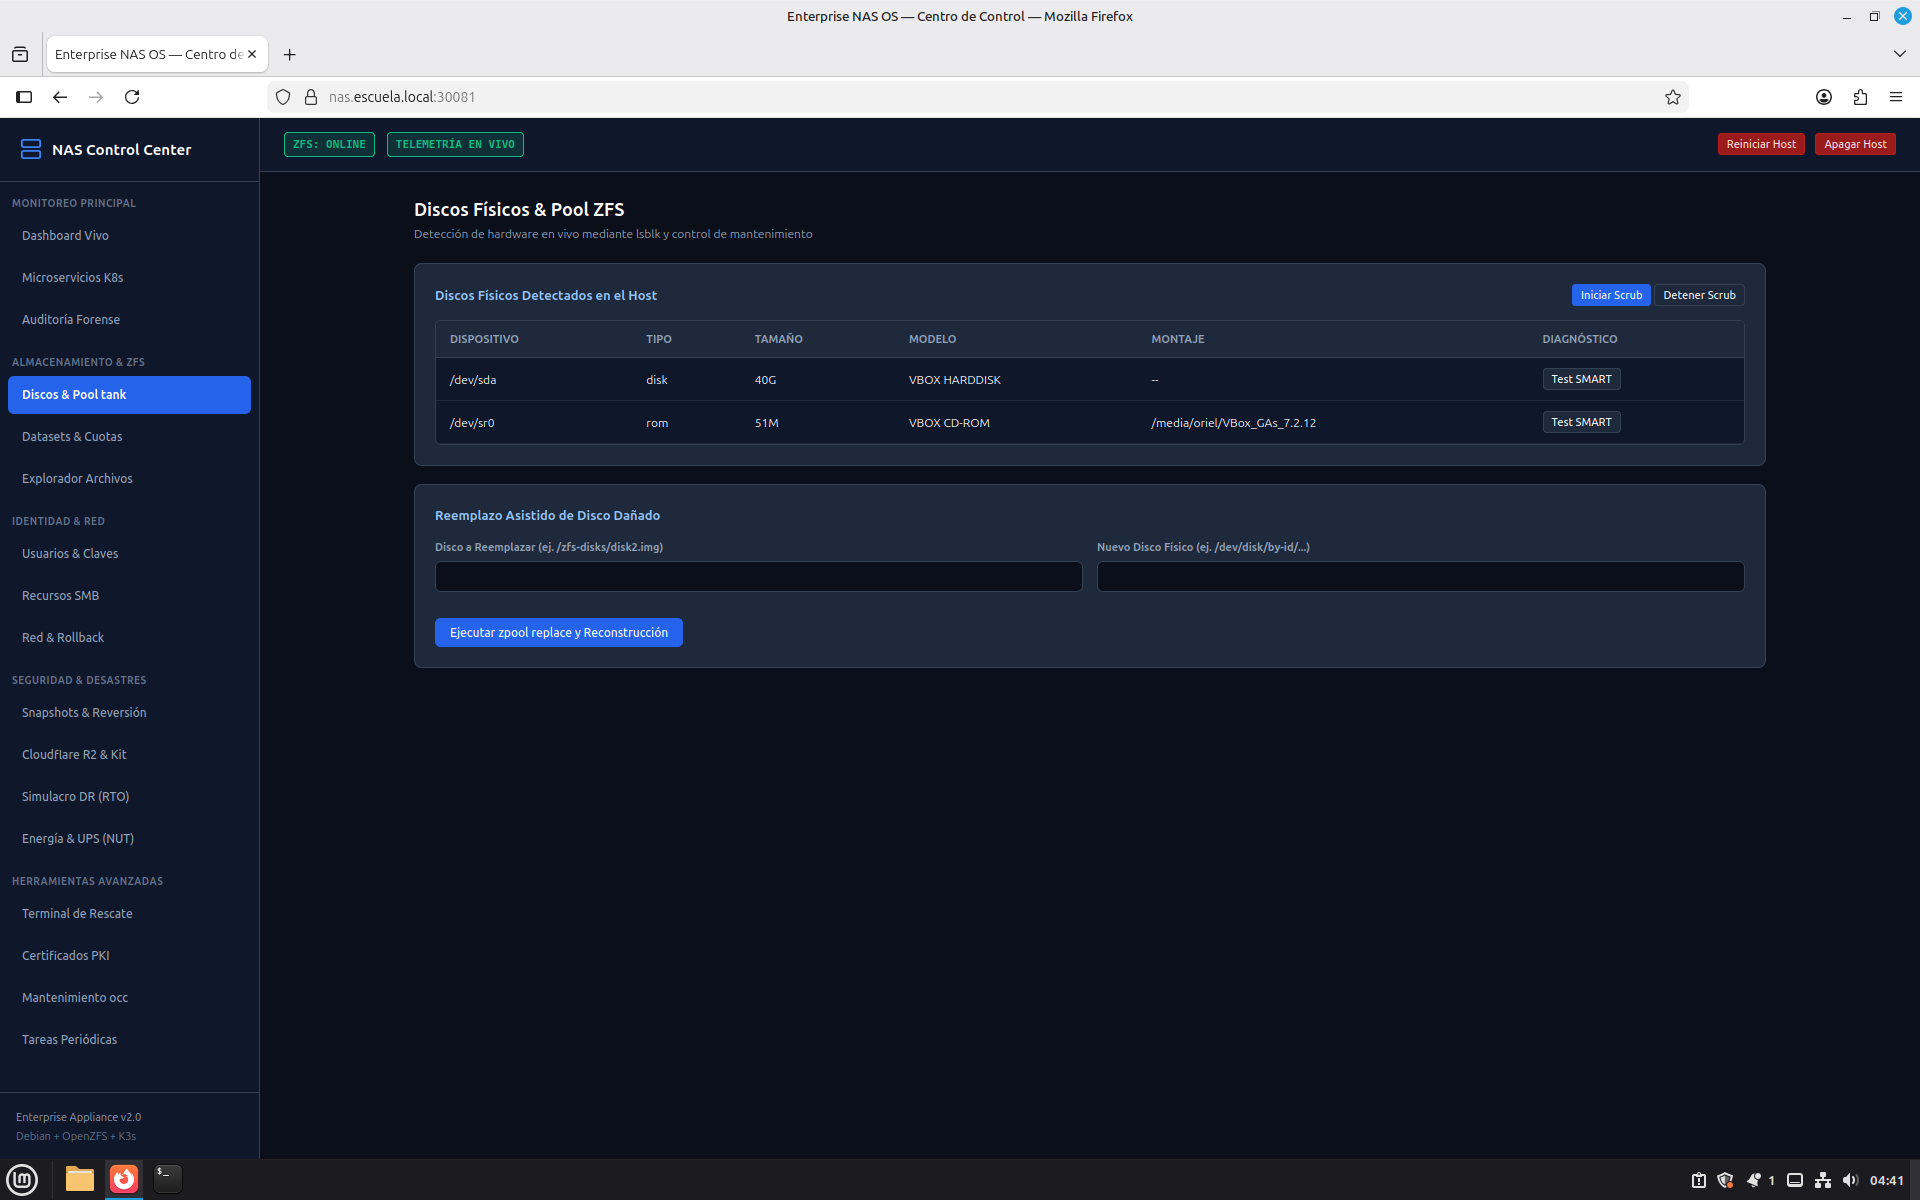
\includegraphics[width=\textwidth]{img/fig02_panel_almacenamiento_zfs.png}
            \tiny Sección de Discos Físicos y Pool ZFS: detección de unidades con \texttt{lsblk}, diagnóstico SMART y reemplazo asistido.
        \end{column}
    \end{columns}
\end{frame}

% ==============================================================================
% DIAPOSITIVA 5: DIMENSIONAMIENTO REAL DE RAM Y DATASET DE RESERVA
% ==============================================================================
\begin{frame}{4. Ingeniería sobre Hardware Real: Memoria RAM y Reserva COW}
    \framesubtitle{Expositor: Oriel Meza — Adaptación a un servidor escolar de 8 GB de RAM}
    \begin{columns}[T]
        \begin{column}{0.49\textwidth}
            \begin{block}{Control de Memoria RAM (Límite ZFS ARC)}
                \footnotesize
                Por defecto, ZFS utiliza hasta el 50\% de la RAM como caché de lectura (\textit{ARC}). En un nodo de 8 GB con contenedores, esto provocaría caídas por falta de memoria (\textit{OOM Killer}).
                \begin{itemize}
                    \item \textbf{Solución:} Fijamos \texttt{zfs\_arc\_max = 2 GB} en \texttt{/etc/modprobe.d/zfs.conf}.
                    \item \textbf{Consumo real medido (30 alumnos):}
                    \begin{itemize}
                        \item Sistema Debian 12: $\approx 600\text{ MB}$
                        \item Caché ZFS ARC (tope): \text{ MB}$
                        \item K3s + Samba + Portal + Sentinel: $\approx 1150\text{ MB}$
                        \item \textbf{Total en carga:} $\mathbf{3,8\text{ GB}}$ ($\mathbf{>4\text{ GB}}$ libres).
                    \end{itemize}
                \end{itemize}
            \end{block}
        \end{column}
        \begin{column}{0.49\textwidth}
            \begin{alertblock}{¿Qué pasa si el disco se llena al 100\% en ZFS?}
                \footnotesize
                Al ser un sistema \textit{Copy-on-Write}, incluso para \textbf{borrar} un archivo (\texttt{rm}) ZFS necesita escribir nuevos metadatos. Si el pool llega al 100\%, el servidor queda bloqueado y no permite borrar nada.
            \end{alertblock}
            \begin{exampleblock}{Solución: Dataset de sacrificio \texttt{tank/buffer}}
                \footnotesize
                Creamos un dataset reservado de \textbf{50 MB} (\texttt{tank/buffer}) sin compresión. Ante una saturación del 100\%, se destruye o vacía esa reserva en 1 segundo para destrabar el pool y limpiar archivos temporales.
            \end{exampleblock}
        \end{column}
    \end{columns}
\end{frame}

% ==============================================================================
% DIAPOSITIVA 6: SERVICIOS ACTIVOS VS STANDBY DECLARATIVO
% ==============================================================================
\begin{frame}{5. Orquestación de Servicios: Producción vs. Standby Declarativo}
    \framesubtitle{Expositor: Oriel Meza — Coherencia entre servicios en ejecución y reserva en GitOps}
    \begin{columns}[T]
        \begin{column}{0.44\textwidth}
            \footnotesize
            \begin{block}{¿Qué es K3s y qué corre en producción?}
                \textbf{K3s} es una distribución ligera de Kubernetes en un solo binario que administra y reinicia automáticamente los contenedores si fallan:
                \begin{itemize}
                    \item \textbf{Samba SMB:} Motor principal de archivos en producción.
                    \item \textbf{Portal QR + TaskEngine:} Consola administrativa web.
                    \item \textbf{Ransomware Sentinel:} Vigilancia de archivos trampa.
                \end{itemize}
            \end{block}
            \begin{block}{¿Por qué Nextcloud está en Standby (L-06)?}
                Los manifiestos de \textbf{Nextcloud y PostgreSQL} están desarrollados y validados en el repositorio, pero se mantienen en \texttt{replicas: 0} en producción para proteger los 8 GB de RAM del host, priorizando el rendimiento de Samba.
            \end{block}
        \end{column}
        \begin{column}{0.54\textwidth}
            \centering
            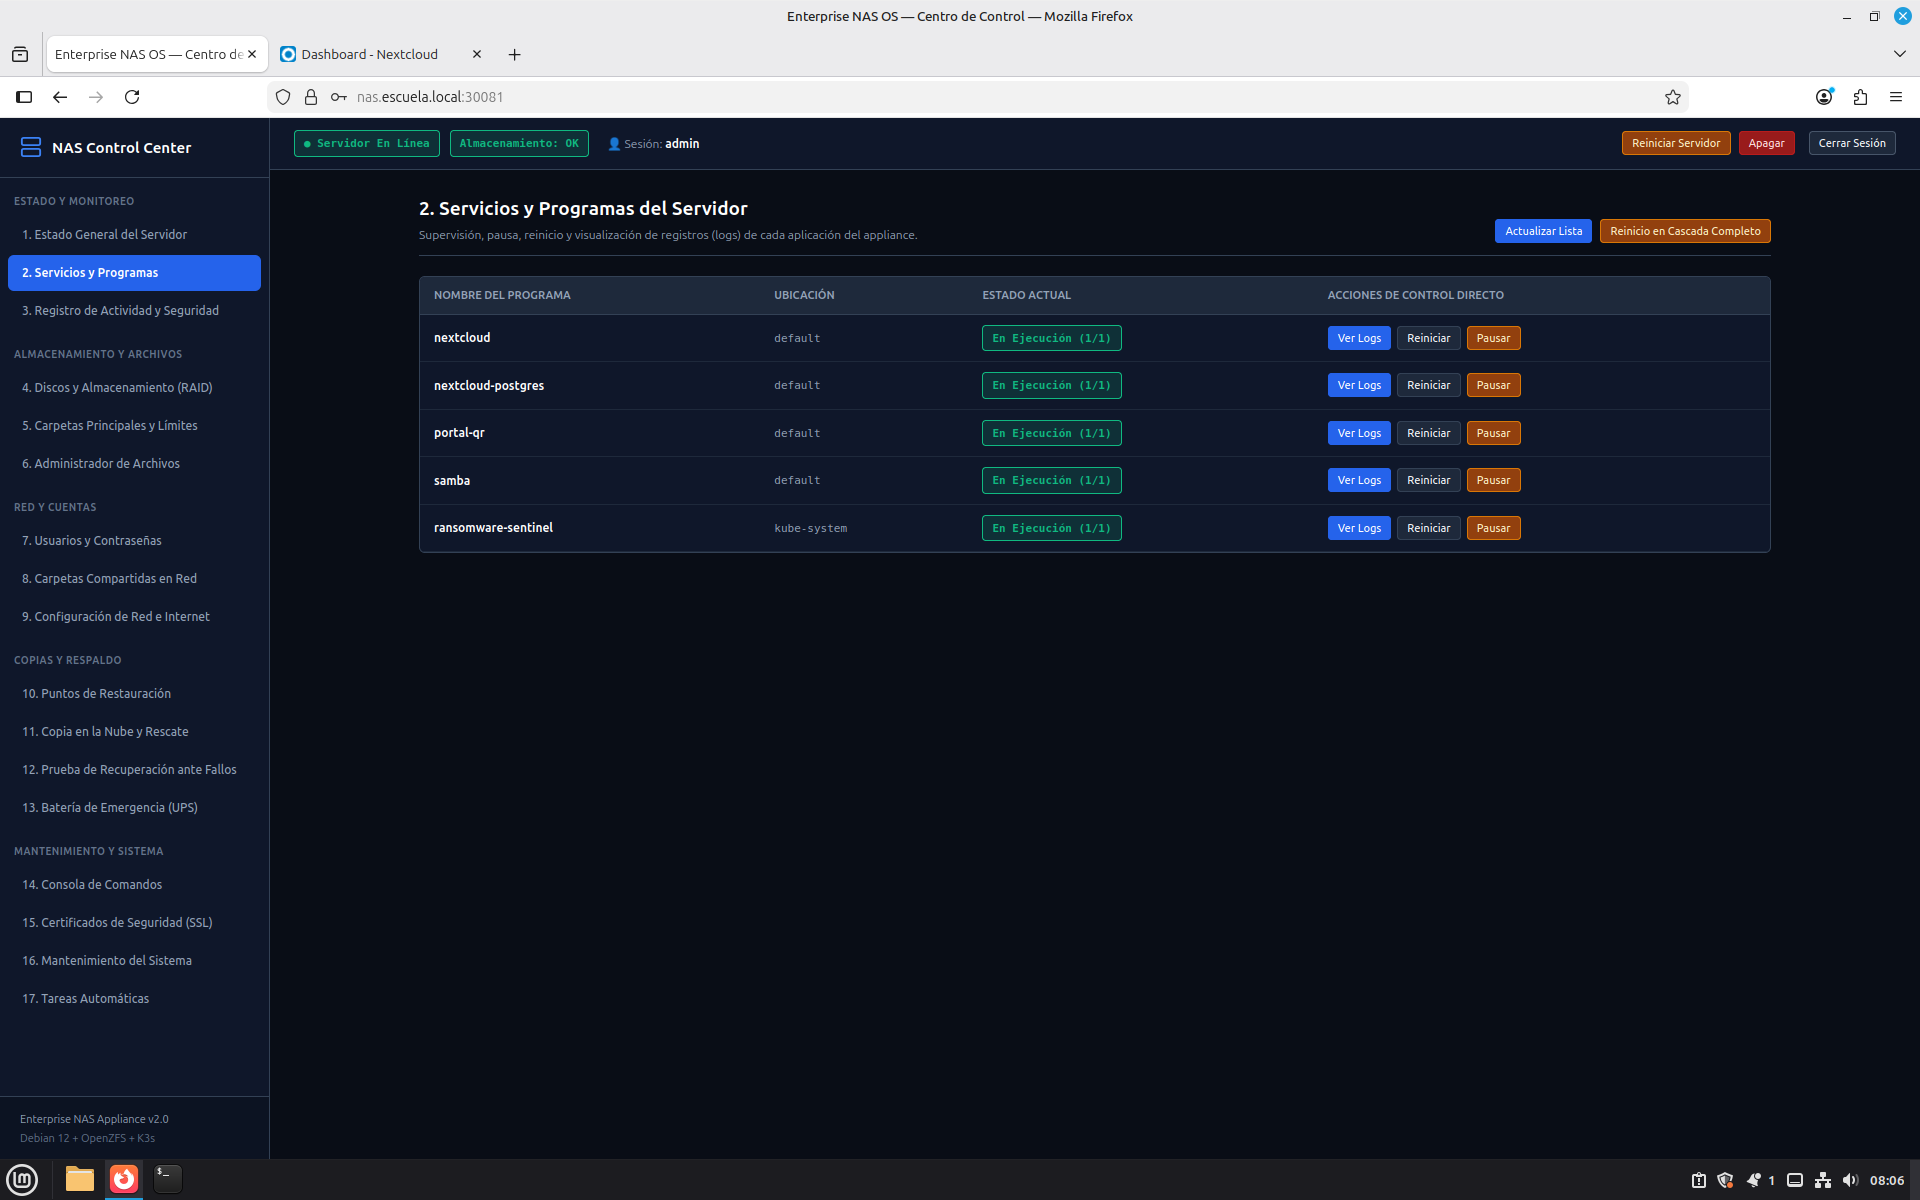
\includegraphics[width=\textwidth]{img/fig06_servicios_activos.png}
            \tiny Sección 2 del Centro de Control: supervisión del estado de ejecución de cada servicio, lectura de logs y reinicio controlado.
        \end{column}
    \end{columns}
\end{frame}

% ==============================================================================
% DIAPOSITIVA 7: ¿QUÉ ES SAMBA Y CÓMO SE ESTRUCTURAN LAS CARPETAS?
% ==============================================================================
\begin{frame}{6. Servicio de Archivos Samba SMB y Estructura de Carpetas}
    \framesubtitle{Expositor: Oriel Meza — Acceso desde red local y administración de permisos}
    \begin{columns}[T]
        \begin{column}{0.44\textwidth}
            \footnotesize
            \begin{block}{¿Qué es Samba (Protocolo SMB/CIFS)?}
                Es la implementación libre del protocolo de red de Microsoft Windows. Permite montar las carpetas del servidor Linux directamente en el Explorador de Windows (\texttt{\textbackslash\textbackslash nas.escuela.local}) como unidades de red sin instalar software adicional en las PCs del aula.
            \end{block}
            \begin{itemize}
                \item \texttt{/tank/nas/docentes}: Material pedagógico (lectura/escritura para profesores).
                \item \texttt{/tank/nas/alumnos/entregas}: Buzón ciego de entrega de trabajos prácticos.
                \item \texttt{/tank/nas/multimedia}: Dataset con bloques de \texttt{1M} para videos educativos.
            \end{itemize}
        \end{column}
        \begin{column}{0.54\textwidth}
            \centering
            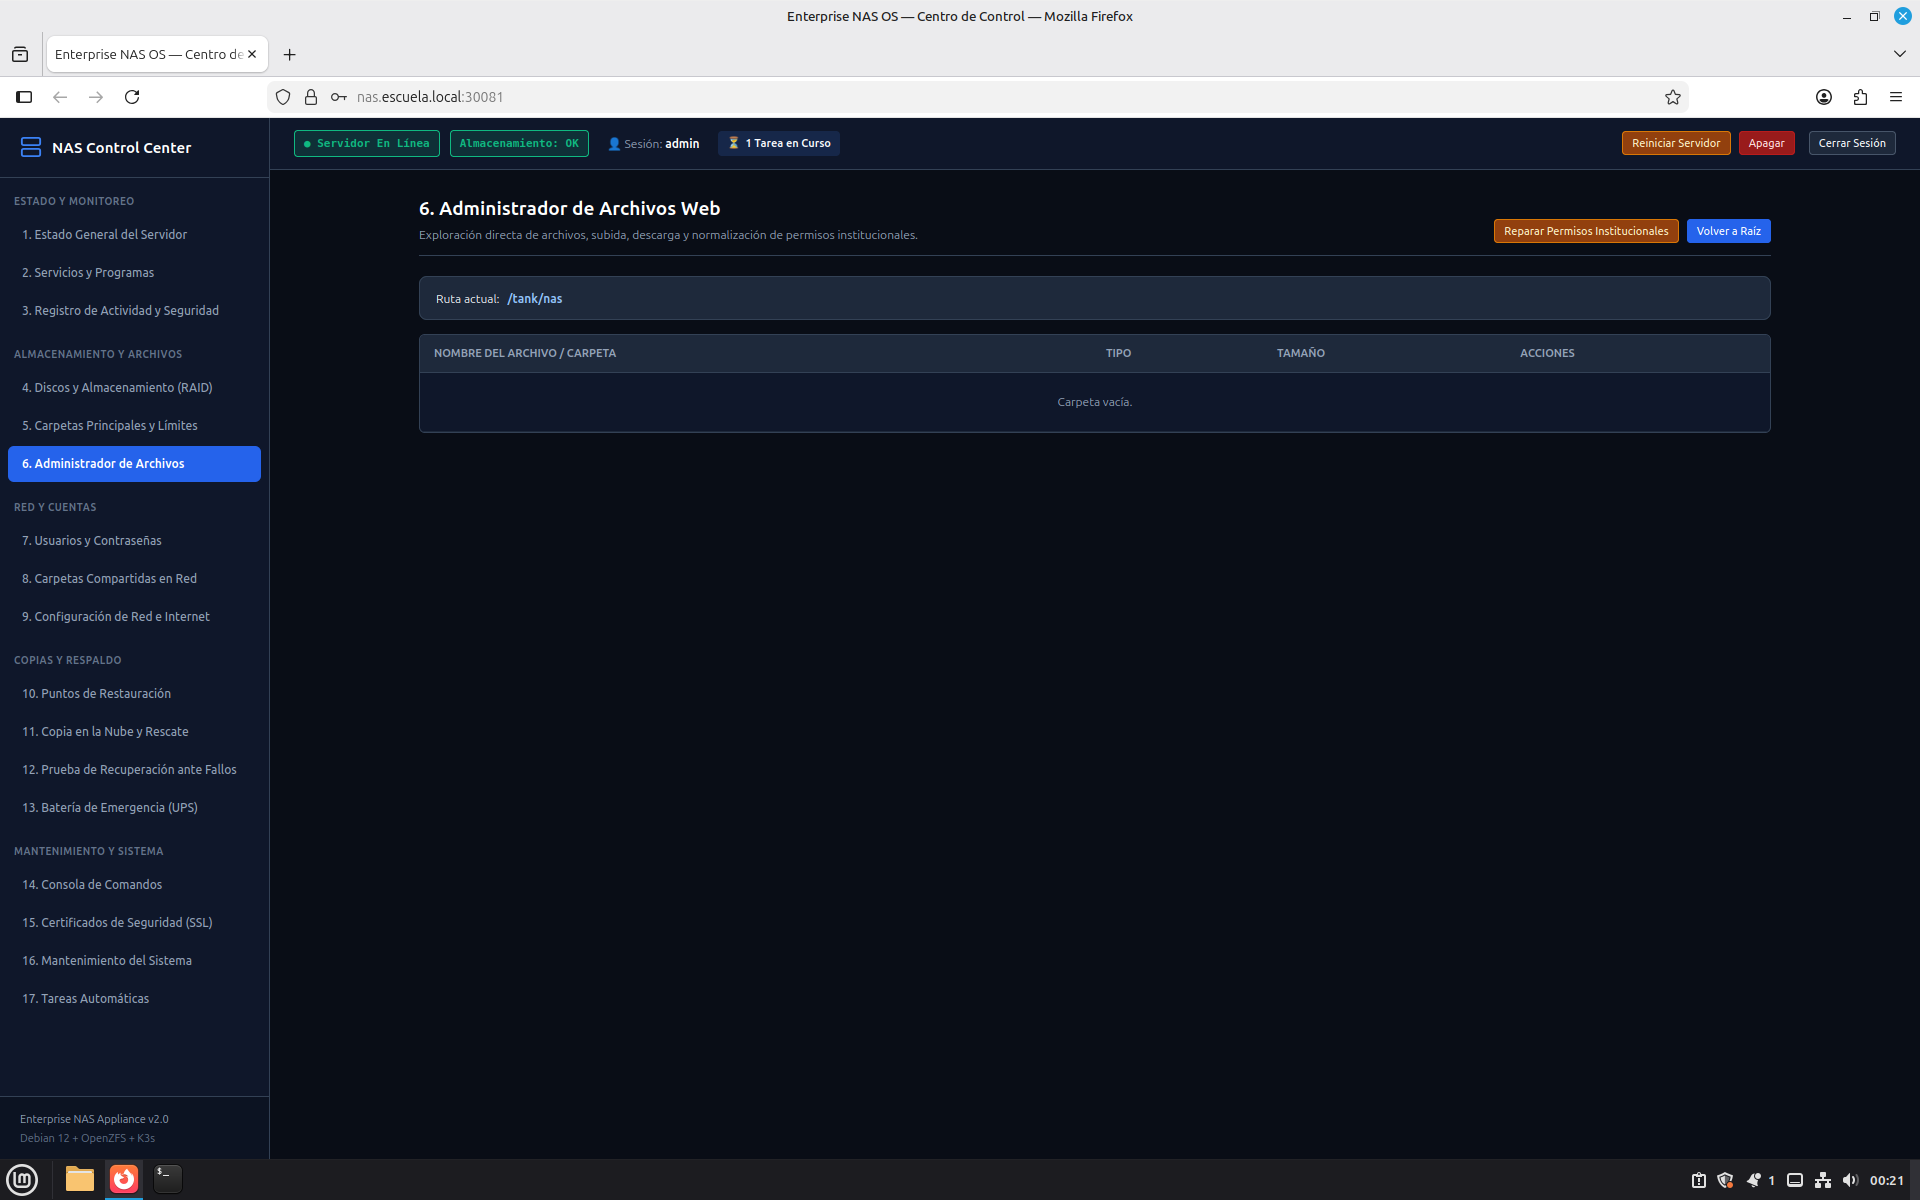
\includegraphics[width=\textwidth]{img/fig09_explorador_archivos_web.png}
            \tiny Sección 6 del Centro de Control: Explorador directo de \texttt{/tank/nas} y botón de normalización automática de permisos POSIX.
        \end{column}
    \end{columns}
\end{frame}

% ==============================================================================
% DIAPOSITIVA 8: EVIDENCIA SAMBA: BUZÓN CIEGO 1777, VETO FILES Y VSS
% ==============================================================================
\begin{frame}{7. Funcionamiento de Samba: Buzón Ciego (1777), Veto Files y VSS}
    \framesubtitle{Expositor: Oriel Meza — Demostración de permisos, bloqueo de malware y snapshots}
    \begin{columns}[T]
        \begin{column}{0.38\textwidth}
            \footnotesize
            \begin{itemize}
                \item \textbf{Buzón Ciego (\texttt{chmod 1777}):} El \textit{Sticky Bit} permite a cada alumno depositar su TP en \texttt{entregas}, pero el kernel impide que un alumno borre o sobrescriba el archivo de otro compañero.
                \item \textbf{Filtro \texttt{veto files}:} Samba rechaza en el acto cualquier intento de copiar archivos ejecutables (\texttt{.exe}, \texttt{.bat}, \texttt{.msi}, \texttt{.ps1}, \texttt{.vbs}).
                \item \textbf{Snapshots ZFS a Windows VSS:} Cada instantánea \texttt{@GMT} generada en ZFS aparece automáticamente en la pestaña \textit{Versiones anteriores} de Windows.
            \end{itemize}
        \end{column}
        \begin{column}{0.60\textwidth}
            \centering
            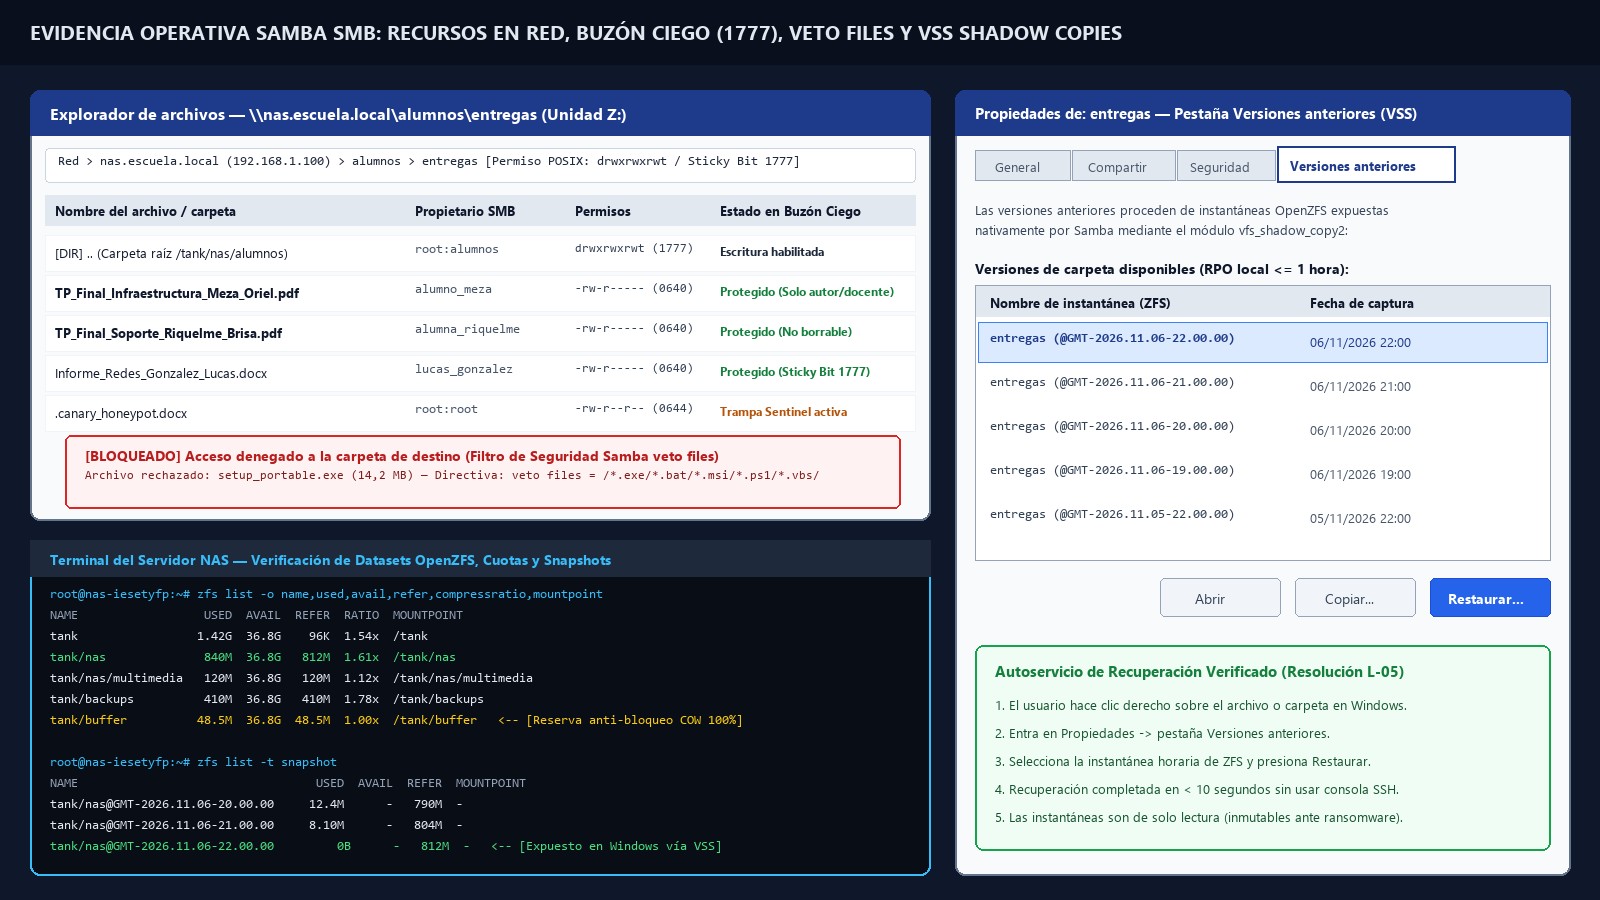
\includegraphics[width=\textwidth]{img/fig07_samba_almacenamiento_vss.png}
            \tiny Evidencia integrada: Explorador de Windows en el recurso SMB, bloqueo \texttt{veto files}, datasets ZFS y pestaña \textit{Versiones anteriores} (VSS).
        \end{column}
    \end{columns}
\end{frame}

% ==============================================================================
% DIAPOSITIVA 9: ADMINISTRACIÓN DE USUARIOS Y PERMISOS
% ==============================================================================
\begin{frame}{8. Administración de Usuarios, Grupos y Contraseñas}
    \framesubtitle{Expositora: Brisa Riquelme — Gestión de identidades y roles institucionales}
    \begin{columns}[T]
        \begin{column}{0.43\textwidth}
            \footnotesize
            \begin{block}{Gestión centralizada sin usar consola}
                Desde la sección \textbf{7. Usuarios y Contraseñas}, el personal técnico o preceptor puede:
                \begin{itemize}
                    \item Dar de alta nuevos usuarios asignándolos a su grupo (\texttt{alumnos}, \texttt{docentes}, \texttt{directivos}).
                    \item Aplicar automáticamente los permisos de red correspondientes a su rol.
                    \item Restablecer contraseñas olvidadas en el aula en segundos o suspender cuentas.
                \end{itemize}
            \end{block}
            \vspace{0.1cm}
            \textbf{Seguridad de acceso:} El portal bloquea automáticamente la dirección IP tras 5 intentos fallidos consecutivos en 5 minutos para frenar ataques de fuerza bruta en la LAN escolar.
        \end{column}
        \begin{column}{0.55\textwidth}
            \centering
            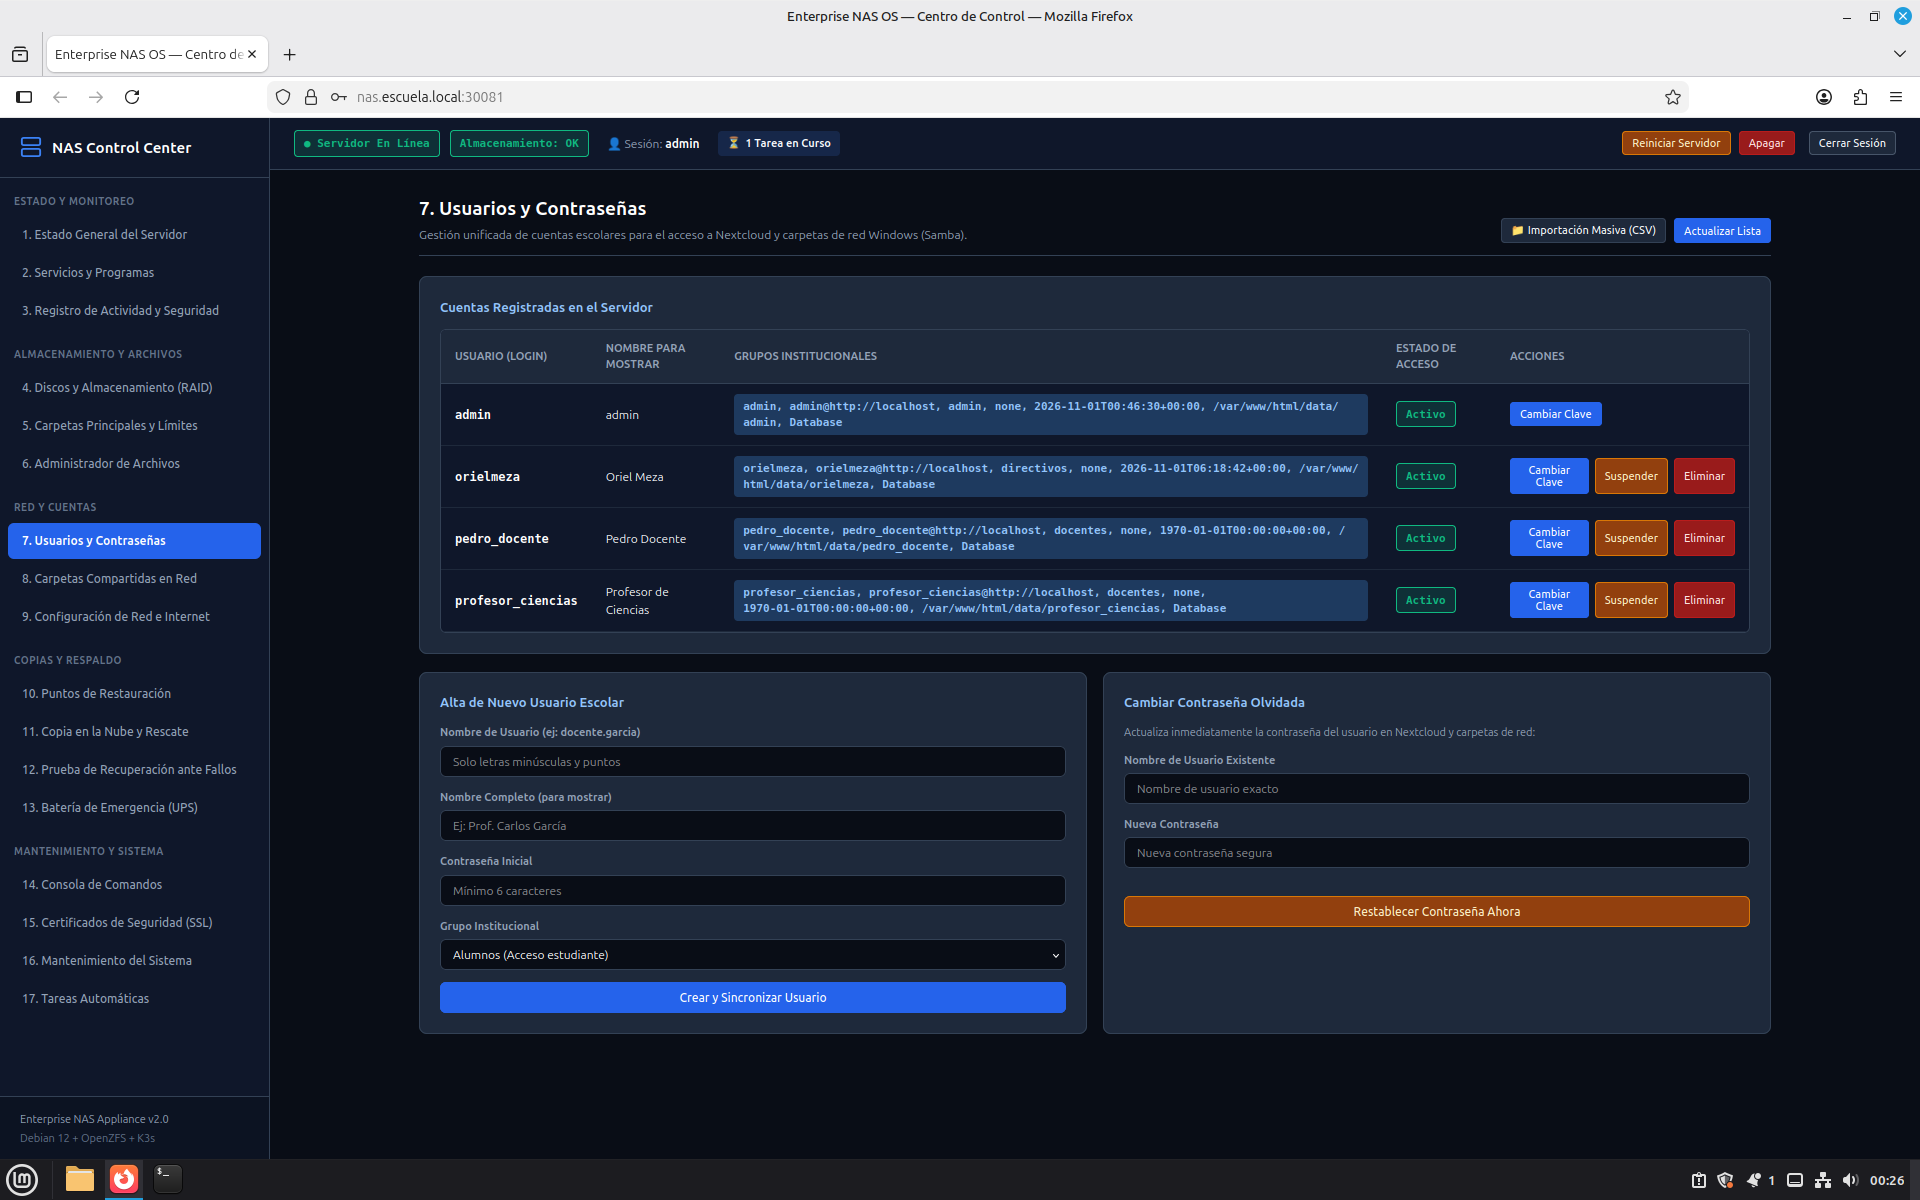
\includegraphics[width=\textwidth]{img/fig03_gestion_usuarios_permisos.png}
            \tiny Sección 7 del Centro de Control: listado de cuentas registradas (\texttt{admin}, \texttt{orielmeza}, \texttt{pedro\_docente}, \texttt{profesor\_ciencias}), estado y acciones.
        \end{column}
    \end{columns}
\end{frame}

% ==============================================================================
% DIAPOSITIVA 10: IMPORTACIÓN MASIVA CSV Y MOTOR TASKENGINE
% ==============================================================================
\begin{frame}{9. Alta Masiva por CSV y Motor Asíncrono \texttt{TaskEngine}}
    \framesubtitle{Expositora: Brisa Riquelme — Automatización de cargas de trabajo pesadas}
    \begin{columns}[T]
        \begin{column}{0.49\textwidth}
            \centering
            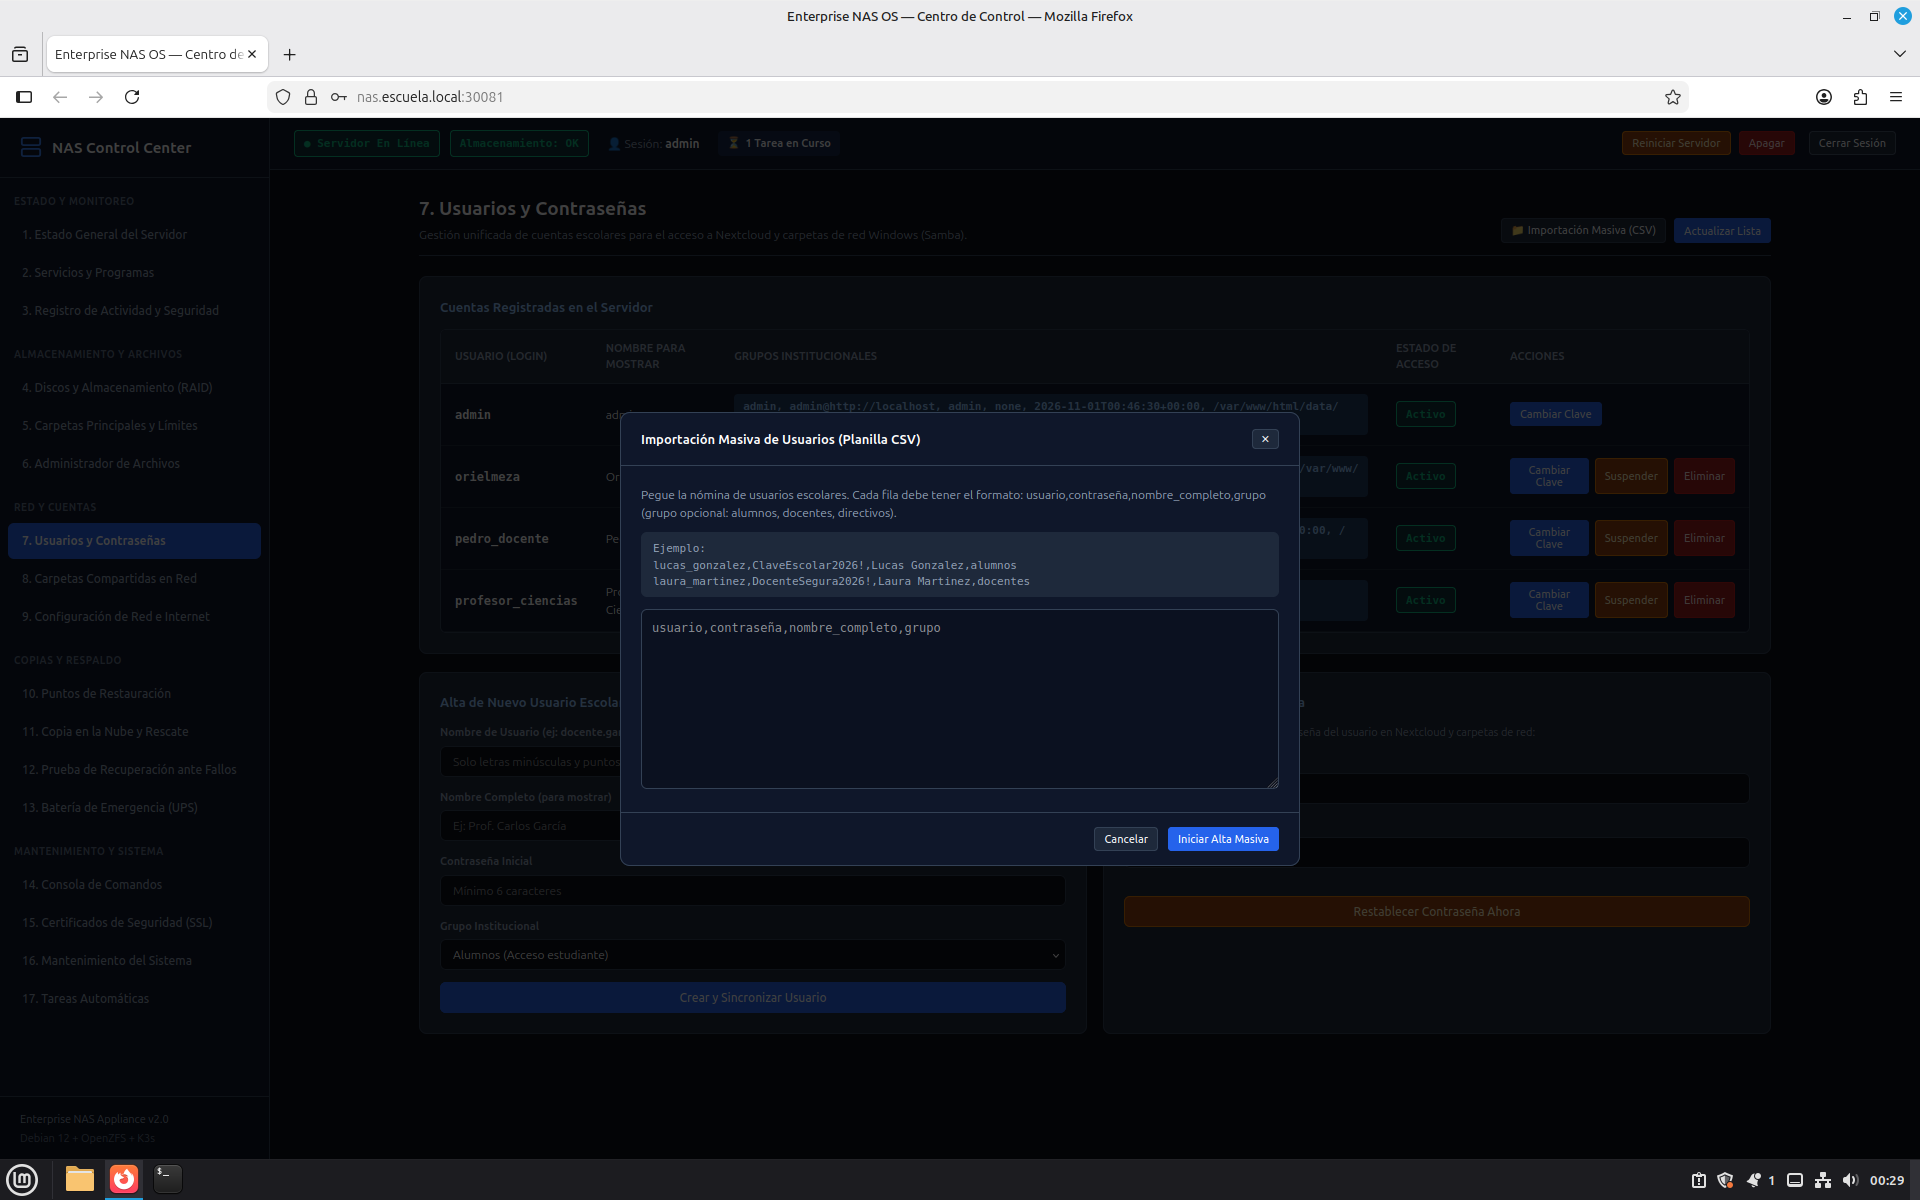
\includegraphics[width=0.95\textwidth]{img/fig05_aprovisionamiento_csv.png}
            \footnotesize
            \textbf{Importación Masiva por Lote (CSV):}\\
            Permite dar de alta divisiones enteras al inicio del ciclo lectivo cargando líneas con formato \texttt{usuario,clave,nombre,grupo}.
        \end{column}
        \begin{column}{0.49\textwidth}
            \centering
            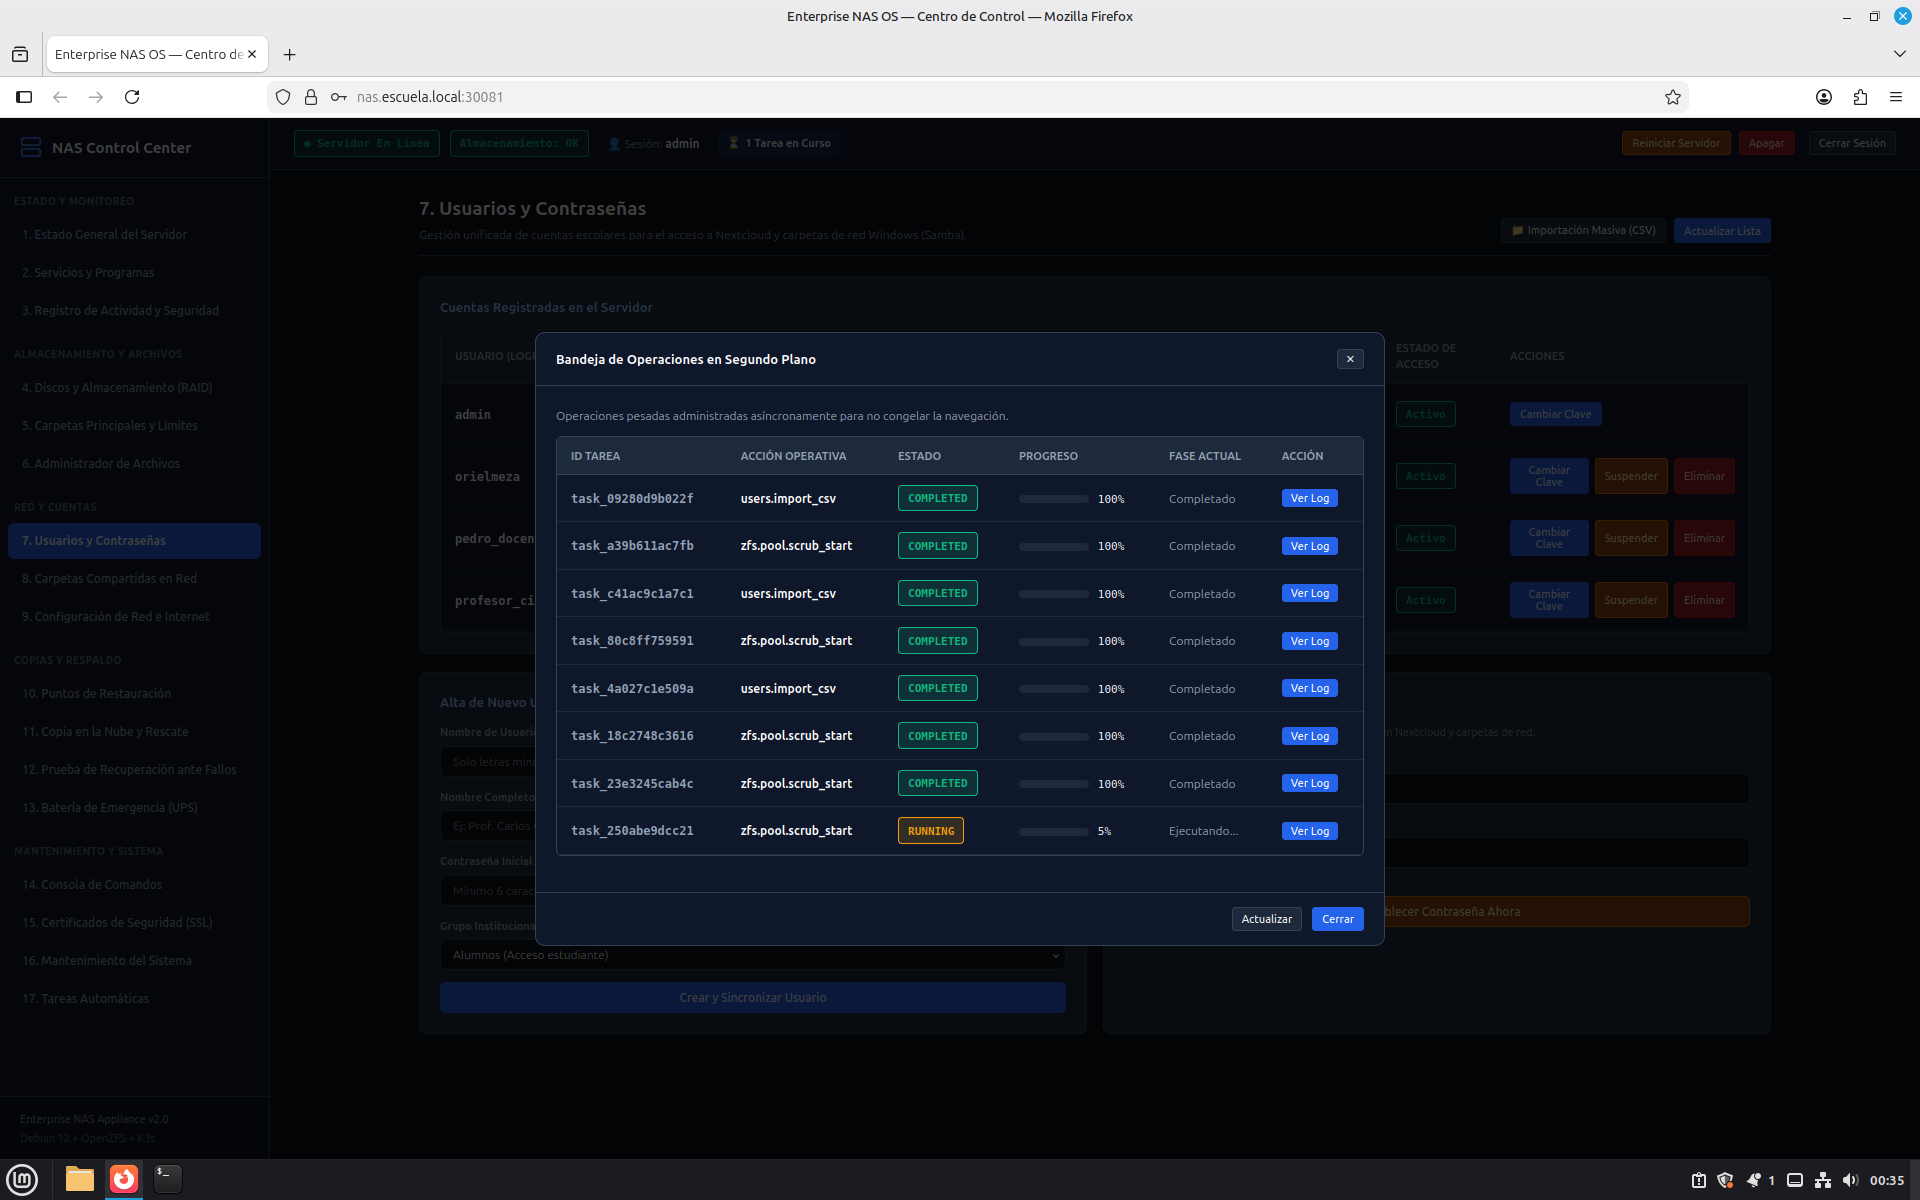
\includegraphics[width=0.95\textwidth]{img/fig04_taskengine_cola_asincrona.png}
            \footnotesize
            \textbf{¿Qué es \texttt{TaskEngine}?}\\
            Motor de cola asíncrona en segundo plano: ejecuta tareas lentas (\texttt{users.import\_csv}, \texttt{zfs.pool.scrub\_start}) sin congelar la interfaz web y guarda el log de auditoría.
        \end{column}
    \end{columns}
\end{frame}

% ==============================================================================
% DIAPOSITIVA 11: ESTRATEGIA DE RESPALDO 3-2-1, CLOUDFLARE R2 Y SENTINEL
% ==============================================================================
\begin{frame}{10. Continuidad Operativa: Regla 3-2-1, Cloudflare R2 y Sentinel}
    \framesubtitle{Expositora: Brisa Riquelme — Respaldo local, externo cifrado y defensa anti-ransomware}
    \begin{columns}[T]
        \begin{column}{0.49\textwidth}
            \begin{block}{Aplicación de la Regla de Respaldo 3-2-1}
                \footnotesize
                \begin{enumerate}
                    \item \textbf{Copia 1 (Producción redundante):} Pool OpenZFS en RAID-Z1 tolerante a la falla de 1 disco físico.
                    \item \textbf{Copia 2 (Instantáneas locales):} Snapshots automáticos cada 1 hora con retención de 30 días ($\text{RPO local} \le 1\text{ h}$), restaurables desde Windows Explorer (VSS).
                    \item \textbf{Copia 3 (Respaldo externo en la nube):} Exportación incremental diaria mediante \texttt{nas-backup.sh} cifrada en origen con \textbf{AES-256-CBC} hacia almacenamiento \textbf{Cloudflare R2}.
                \end{enumerate}
            \end{block}
        \end{column}
        \begin{column}{0.49\textwidth}
            \begin{alertblock}{Custodia externa de claves maestras}
                \footnotesize
                Si el servidor físico sufriera destrucción total, el backup en la nube sería inútil sin la llave de descifrado. Por ello, las claves se exportan con \texttt{export-master-keys.sh} a un medio externo bajo custodia fuera del servidor (\textbf{RTO ante desastre total $\le 2\text{ h}$}).
            \end{alertblock}
            \begin{exampleblock}{¿Qué es el demonio \texttt{Sentinel}?}
                \footnotesize
                Servicio que vigila archivos trampa (\texttt{.canary\_honeypot.docx}) mediante eventos \texttt{inotify} del kernel. Si un ransomware los modifica, aplica \texttt{zfs hold} para impedir el borrado de snapshots.
            \end{exampleblock}
        \end{column}
    \end{columns}
\end{frame}

% ==============================================================================
% DIAPOSITIVA 12: VALIDACIÓN CI/CD EN GITHUB ACTIONS Y SECRETOS CIFRADOS
% ==============================================================================
\begin{frame}{11. Validación del Repositorio (GitHub Actions CI) y Sealed Secrets}
    \framesubtitle{Expositor: Oriel Meza — Corrección de errores de YAML y validación de manifiestos}
    \begin{columns}[T]
        \begin{column}{0.41\textwidth}
            \footnotesize
            \begin{block}{¿Qué son Sealed Secrets y el pipeline CI?}
                \begin{itemize}
                    \item \textbf{Sealed Secrets:} Cifra las contraseñas de Kubernetes para poder guardarlas en GitHub sin exponer ninguna clave en texto plano.
                    \item \textbf{Corrección realizada en CI:}
                    \begin{enumerate}
                        \item Se eliminó el atributo inválido \texttt{creationTimestamp: null} de los 4 manifiestos \texttt{SealedSecret} que hacía fallar a \texttt{kubeconform}.
                        \item Se normalizaron los saltos de línea CRLF a formato UNIX (\texttt{LF}) y se configuró \texttt{.yamllint}.
                    \end{enumerate}
                \end{itemize}
            \end{block}
        \end{column}
        \begin{column}{0.57\textwidth}
            \centering
            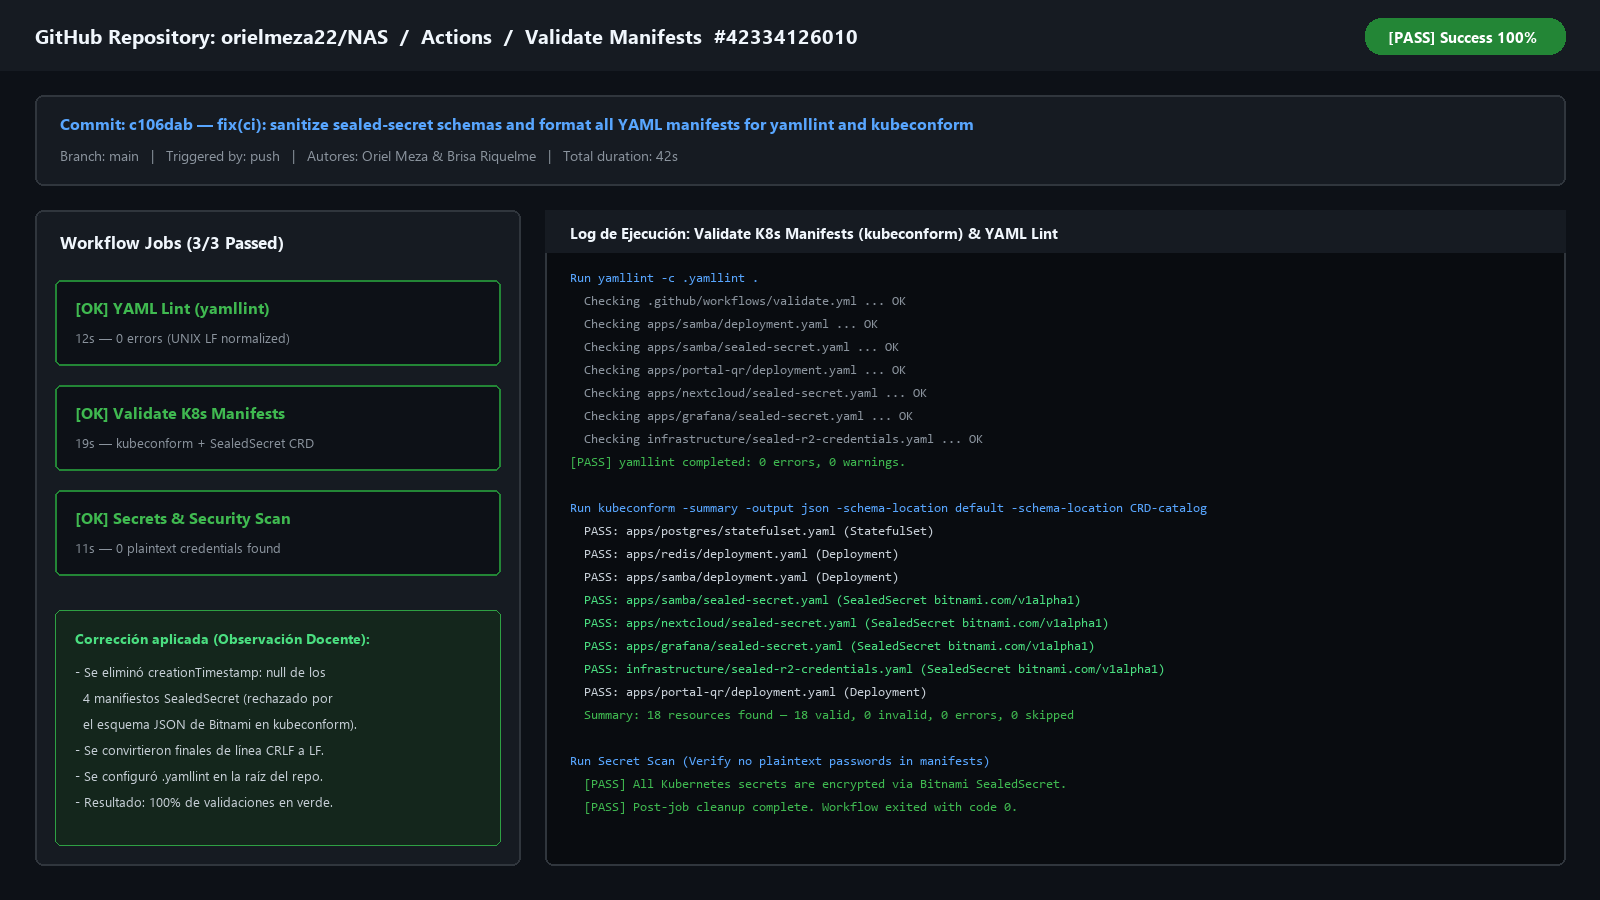
\includegraphics[width=\textwidth]{img/fig08_github_actions_ci.png}
            \tiny Ejecución exitosa (100\% en verde) de los 3 trabajos de validación en GitHub Actions (\texttt{YAML Lint}, \texttt{Validate K8s Manifests} y \texttt{Secrets Scan}).
        \end{column}
    \end{columns}
\end{frame}

% ==============================================================================
% DIAPOSITIVA 13: REGISTRO DE FALLAS DETECTADAS Y SOLUCIONES APLICADAS
% ==============================================================================
\begin{frame}{12. Pruebas de Laboratorio: Fallas Detectadas y Soluciones}
    \framesubtitle{Expositor: Oriel Meza — Transparencia técnica y resolución de problemas reales}
    \footnotesize
    \begin{table}
        \centering
        \begin{tabular}{|c|p{3.6cm}|p{4.4cm}|p{5.2cm}|}
            \hline
            \textbf{N.º} & \textbf{Incidencia detectada} & \textbf{Causa raíz identificada} & \textbf{Solución técnica aplicada} \\
            \hline
            1 & Error en GitHub Actions (\texttt{kubeconform} y \texttt{yamllint}). & Campo \texttt{creationTimestamp: null} en SealedSecrets y saltos de línea CRLF. & Saneamiento de los 4 manifiestos cifrados, conversión a LF y configuración de \texttt{.yamllint}. \\
            \hline
            2 & Archivos de Samba no se guardaban en el pool ZFS. & El volumen \texttt{samba-pvc} apuntaba a una carpeta temporal \texttt{local-path} (ext4). & Vinculación explícita a \texttt{/tank/nas} con directiva \texttt{mountPropagation: HostToContainer}. \\
            \hline
            3 & El contenedor Samba ignoraba la regla \texttt{veto files}. & El script de inicio de la imagen Docker sobrescribía \texttt{smb.conf} al arrancar. & Inyección de la variable \texttt{VETO=no} en \texttt{deployment.yaml}, activando el bloqueo de \texttt{.exe} y scripts. \\
            \hline
            4 & Riesgo de saturación de los 8 GB de RAM del servidor. & ZFS ARC tomaba 4 GB por defecto y Nextcloud + Postgres sumaban $>2\text{ GB}$. & Tope de ZFS ARC en 2 GB y pase de Nextcloud a modo \textit{standby declarativo} (\texttt{replicas: 0}). \\
            \hline
            5 & Bloqueo de comando \texttt{rm} al llenar el disco al 100\%. & En Copy-on-Write borrar requiere espacio libre para escribir metadatos nuevos. & Creación del dataset de reserva \texttt{tank/buffer} (50 MB) liberable en caso de emergencia. \\
            \hline
        \end{tabular}
    \end{table}
\end{frame}

% ==============================================================================
% DIAPOSITIVA 14: DEMOSTRACIÓN PRÁCTICA Y CONCLUSIONES
% ==============================================================================
\begin{frame}{13. Conclusiones y Demostración Práctica en Vivo}
    \framesubtitle{Exponen: Oriel Meza y Brisa Riquelme — Cierre y ronda de preguntas}
    \begin{columns}[T]
        \begin{column}{0.48\textwidth}
            \begin{block}{Recorrido de la Demostración en Vivo}
                \footnotesize
                \begin{enumerate}
                    \item \textbf{Verificación de salud (Oriel):} Estado del pool \texttt{tank} en RAID-Z1 y servicios activos en el Centro de Control.
                    \item \textbf{Acceso SMB y permisos (Oriel):} Subida de trabajo práctico al buzón ciego (\texttt{1777}) y prueba de bloqueo de un archivo \texttt{.exe} (\texttt{veto files}).
                    \item \textbf{Gestión de usuarios y CSV (Brisa):} Alta de usuario escolar y monitoreo en \texttt{TaskEngine}.
                    \item \textbf{Respaldo y restauración VSS (Brisa):} Borrado accidental de un archivo y recuperación inmediata desde \textit{Versiones anteriores}.
                \end{enumerate}
            \end{block}
        \end{column}
        \begin{column}{0.48\textwidth}
            \begin{exampleblock}{Resultados Consolidados del TIF}
                \footnotesize
                \begin{itemize}
                    \item \textbf{18/18 casos de prueba (TC-01 a TC-18)} verificados y documentados bajo normas ISO.
                    \item \textbf{Consumo de recursos controlado:} ,8\text{ GB}$ de RAM en concurrencia sobre \text{ GB}$ físicos.
                    \item \textbf{Continuidad garantizada:} $\text{RPO local} \le 1\text{ h}$, $\text{RTO} \le 35\text{ min}$ con pool intacto y copia cifrada en la nube.
                \end{itemize}
            \end{exampleblock}
            \vspace{0.2cm}
            \centering
            \textbf{\large ¡Muchas gracias por su atención!}\\
            \footnotesize Quedamos a disposición para preguntas de la cátedra y compañeros.\\
            \textbf{Oriel Meza y Brisa Riquelme} — Soporte Técnico II (IESETyFP)
        \end{column}
    \end{columns}
\end{frame}

\end{document}
